\documentclass[crop,tikz,european resistors]{standalone}
\usepackage{circuitikz}[european]
\begin{document}
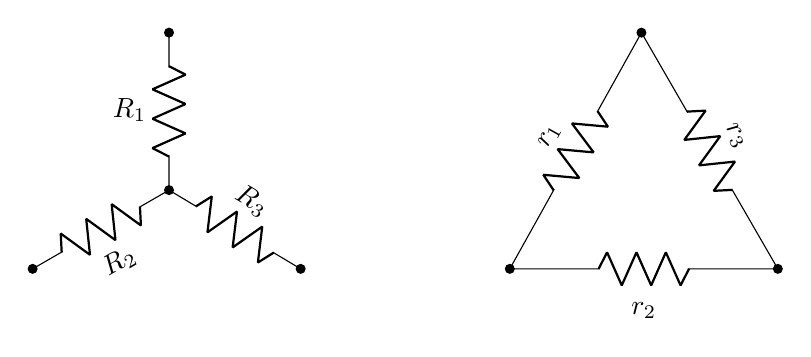
\begin{tikzpicture}
    \draw (-3,0) to[R=$R_1$, *-*] (-3, 2);
    \draw (-3,0) to[R=$R_2$, -*] (-4.732,-1);
    \draw (-3,0) to[R=$R_3$, -*] (-1.328,-1);

    \draw (3,2) to[R=$r_3$, -*] (4.732,-1);
    \draw (4.732,-1) to[R=$r_2$, -*] (1.328,-1);
    \draw (1.328,-1) to[R=$r_1$, -*] (3,2);
\end{tikzpicture}
\end{document}
